\chapter{Theory of Operation} 
\label{theory}  
\section{Nuclear Polarization}
In the presence of a magnetic field, spin-\half{} nuclei tend to align themselves along the axis of the field.  The polarization of the ensemble of particles is defined by 

\begin{eqnarray}
\label{eqn:polarization-definition}
\mathcal{P}=\frac{N_\uparrow-N_\downarrow}{N_\uparrow+N_\downarrow},
\end{eqnarray}

where $N_\downarrow$ ($N_\uparrow$) is the population of spins with $m_z$ equal to $-$\half{} (+\half).  For simplicity, the remainder of the section assumes particles of spin-\half{}.

\subsection{Thermal Polarization Derivation}


A macroscopically sized target has $N$ particles, where $N$ is very large.  While any spin has exactly equal probability of being $\uparrow$ or $\downarrow$, it is not given that exactly half of $N$ are $\uparrow$.  This is easy to see when considering ten coins dropped on the ground: there is a $\approx$25\% chance that half of them will be heads and a $\approx$75\% chance of another outcome.


The relative odds of the system having $a$ particles $\uparrow$ to the system have $b$ particles $\uparrow$ is interesting.  To simplify notation, we give the name $M_x$ to number of ways of getting $x$ particles $\uparrow$ and call it the \textit{multiplicity} of getting $x$.  Now it becomes apparent that the probability $P_a$ of the system having $a$ spins $\uparrow$ is related to the probability $P_b$ of having $b$ spins $\uparrow$ is

\begin{eqnarray}
 \frac{P_a}{P_b} = \frac{M_a}{M_b},
\end{eqnarray}

since a higher multiplicity is associated with a higher probability for each state.

Using $S=k\ln M$ and other thermodynamic relationships (TODO come back and actually work all this out) we arrive at 

\begin{eqnarray}
 \frac{P_a}{P_b} = \frac{e^{-E_a/kT}}{e^{-E_b/kT}},
\end{eqnarray}

which is known as the Boltzmann factor that relates $P_a$ to $P_b$.  For the spin-\half{} system this gives us the ratios of populations

\begin{eqnarray}
 \frac{N_\downarrow}{N_\downarrow} = \frac{e^{E_\downarrow/kT}}{e^{E_\uparrow/kT}}.
\end{eqnarray}


We are now in position to rewrite the definition of polarization (Equation \ref{eqn:polarization-definition}) in terms of thermodynamic variables:

\begin{eqnarray}
 \mathcal{P}&=&\frac{N_\uparrow}{N_\uparrow+N_\downarrow}-\frac{N_\downarrow}{N_\uparrow+N_\downarrow} \\
 &=& \frac{1}{1+\frac{N_\downarrow}{N_\uparrow}}-\frac{1}{\frac{N_\uparrow}{N_\downarrow}+1} \\
 &=& \frac{1}{1+e^{-\Delta E/kT}}-\frac{1}{1+e^{\Delta E/kT}} \\
 &=& \tanh\left(\frac{\mu H}{kT}\right)
\end{eqnarray}

where $\Delta E\equiv E_\uparrow-E_\downarrow = 2 \mu H$.

 \subsection{DNP}
Dynamic Nuclear Polarization (DNP) is a process of using microwave radiation to pump electron-proton pairs to higher energy (polarized) states.  The relaxation time for the electron is much shorter than that of the proton, so the proton remains polarized while the electron is able to be paired with other protons for polarization.

\begin{figure}
 \centering
 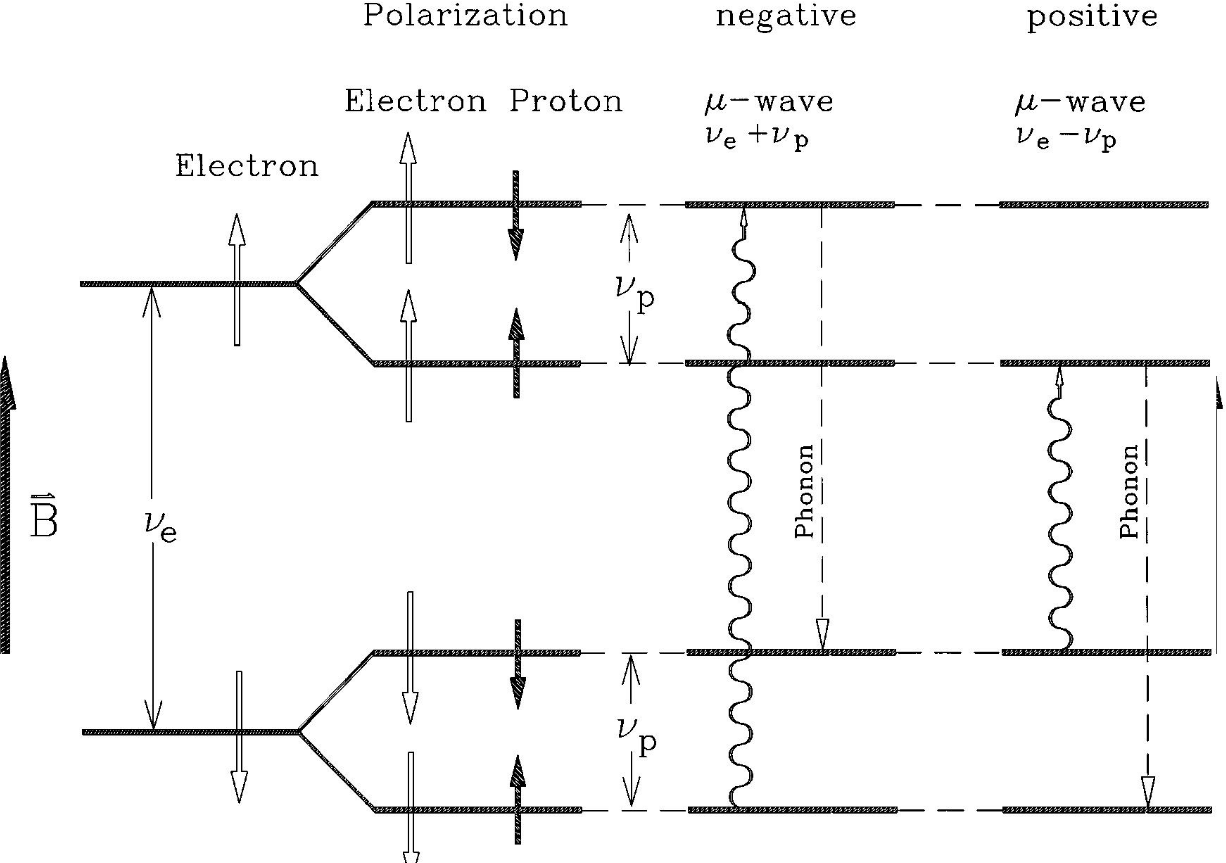
\includegraphics[scale=.25]{img/dnp.png}
 % dnp.png: 1226x863 pixel, 72dpi, 43.25x30.44 cm, bb=0 0 1226 863
 \caption{DNP diagram \cite{dnpdiagram}.  The white arrows are electron polarization and the black arrows are proton polarization.  Microwaves at a frequency difference $\nu_e\pm\nu_p$ flip the spins of both particles, and the electron's superior lattice coupling ensures it will flip back before the proton.}
 \label{fig:dnp-diagram}
\end{figure}


The microwave frequency can either be the sum of the proton and electron splitting frequency or the difference, depending on whether the nucleons are to be aligned with or against the magnetic field. 
\section{NMR}

Nuclear Magnetic Resonance (NMR) is the method we use to measure the polarization of the target material.  Essentially, a coil in the immediate vicinity of the target acts as the inductor in an LCR circuit, the inductance of which changes as a function of the magnetic susceptibility of the nuclei in the coil.  Since the magnetic susceptibility and polarization are related, the resonance frequency of the LCR circuit tell us information about the polarization of the target material\cite{qmeterbook}. 

\subsection{Liverpool Q-Meter}

\subsubsection{$\lambda$/2 Cable}

\subsubsection{Diode Detector}

\subsubsection{Phase Sensitive Detector and BRM}

\subsection{PDP}

\section{Frozen Spin} 
 
 The target is polarized in a 2.5 T field, called the polarizing field, generated from a large, super-conducting magnet (TODO photo).  Without this polarizing field, the target immediately loses all polarization properties.  Since the magnet obstructs the path between the target and detectors, greatly reducing the solid angle available, we wish to employ a method of maintaining target polarization without the polarizing magnet in the way.  The method of choice is Hifrost's namesake frozen spin method.
 
 
 A 0.5 T field, generated from an internal superconducting coil (TODO photo), is ramped up while the target is at maximum polarization.  At dilution temperatures, this smaller field, called the holding field, sufficiently maintains nuclear polarization while the polarizing magnet is removed and the detector is placed around the target (TODO diagram). 
 
 

\section{Refrigerator} 
Since the polarization goes like the inverse of temperature, colder environments make for better polarized targets.  In our case, we use a dilution refrigerator, one that mixes the two isotopes \het{} and \hef{} for cooling, to reach target temperatures below 0.1 K.

\subsection{\hef{}Cooling (Evaporator and Separator)}

\subsection{Dilution}

The dilution refrigerator principle relies on the splitting of a \het/\hef{} mixture into two distinct phases, a \het{} concentrated phase and a \het{} dilute phase.  The area labeled ``Two-phase region'' in Figure \ref{fig:dilutiondiagram} illustrates which mixtures, characterized by \het{} concentration, are inaccessible at which temperatures.  Since two distinct phases in thermal contact are always in or striving for thermodynamic equilibrium, changing the concentration of the dilute phase (by pumping \het{} out of it) will cause atoms from the concentrated phase to cross the phase boundary to restore balance.  Since the heat change of mixing (enthalpy difference between the dilute phase and concentrated phase) is positive, the \het{} crossing the phase boundary must absorb energy from the surrounding environment, which it does in the form of heat.\cite{hocktechniques}

\begin{figure}
 \centering
 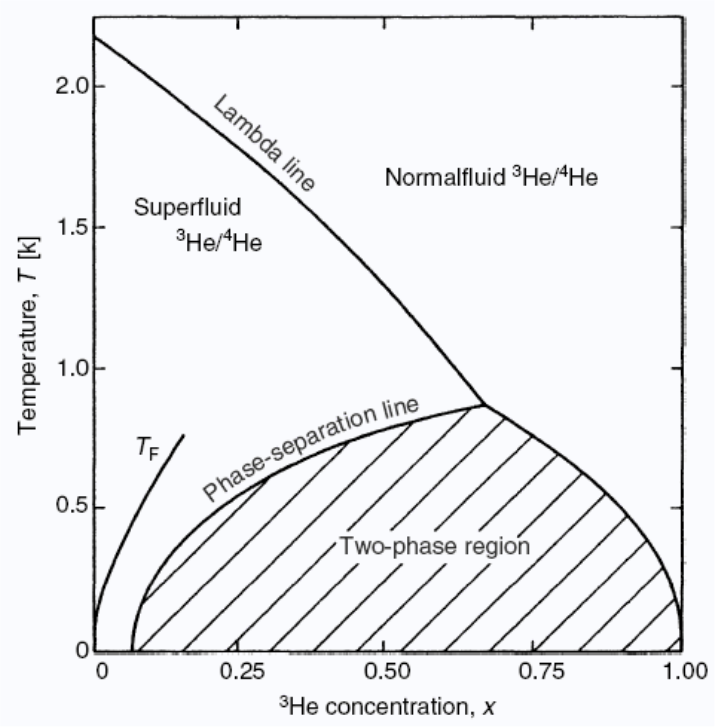
\includegraphics[scale=.45]{img/dilutiondiagram.png}
 % dilutiondiagram.png: 715x727 pixel, 72dpi, 25.22x25.64 cm, bb=0 0 715 727
 \caption{The famous diagram that shows the splitting of two distinct phases of $\het$-$\hef$ mixture. \cite{dilutiondiagram}}
 \label{fig:dilutiondiagram}
\end{figure}
 
